% meta.concepts: distributed load
% meta.tags: realistic
% acknowledge: Peter Seiler & Luke Melander graciously shared Spring 2019 course material
% source: 2019 P. Seiler AEM2011 HW 7

The lift force generated on an aircraft wing is distributed along the span of the wing. Generally the distributed
force is larger near the body of the aircraft and decreases toward the wingtip. A simple diagram showing the
aircraft body (viewed from the front) and one wing is shown below. Treat the wing as rigidly attached to the
aircraft body and assume the distributed lift force is given by an ellipitical profile for $x \le 3$m:
\begin{equation*}
  f(x) = \sqrt{9-x^2} N/m
\end{equation*}
Find:
\begin{enumerate}
  \item The magnitude and location of the resultant of the distributed load.
  \item The support reaction applied by the aircraft body on the aircraft wing at $x = 0$.
\end{enumerate}

\begin{figure}[ht!]
  \centering
  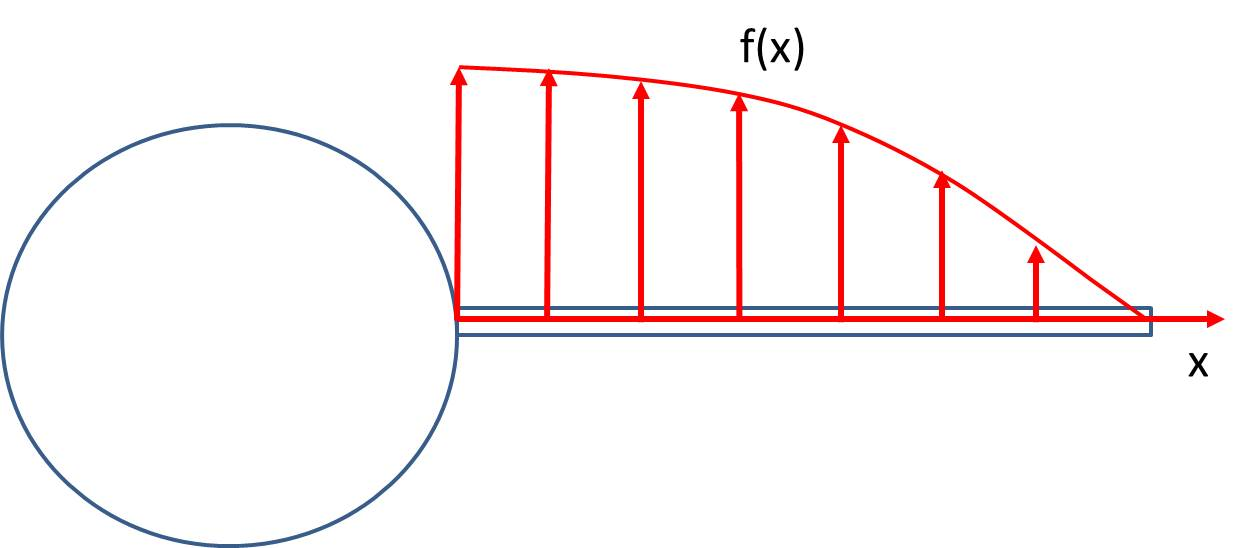
\includegraphics[height=1.8in]{fig.png}
  \caption*{Simplified diagram of wing loading.}
\end{figure}

\iftoggle{flagSoln}{%
\vspace{.5cm}
\rule{\textwidth}{.4pt}
\vspace{.5cm}
\textbf{Solution:}
\begin{figure}[ht!]
  \centering
  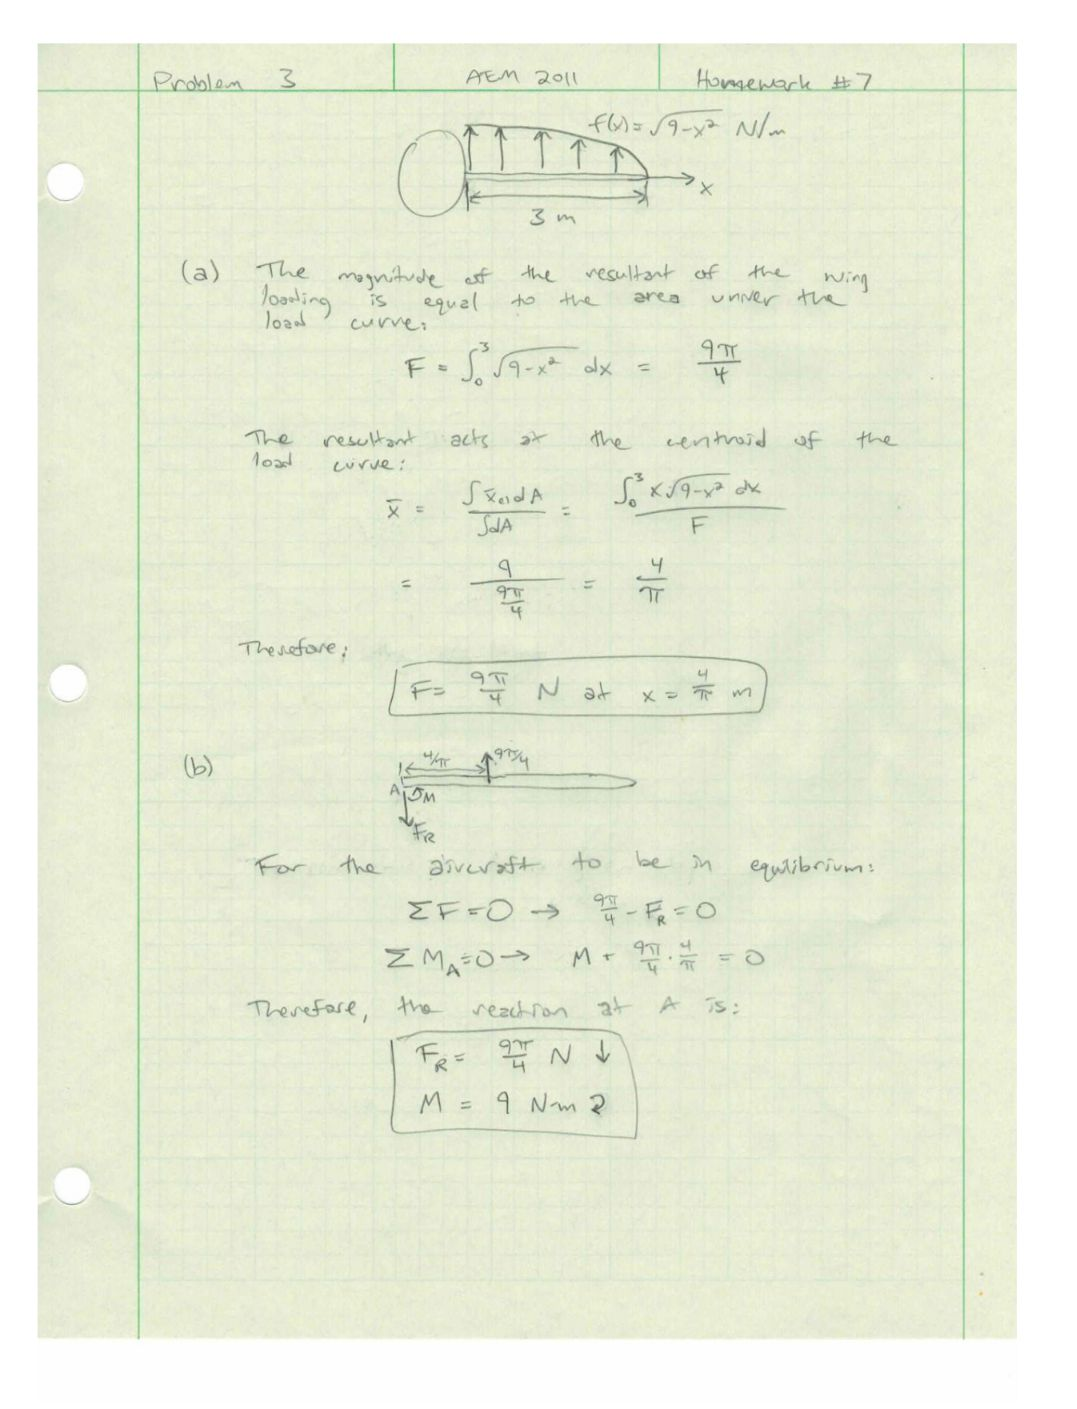
\includegraphics[width=0.9\textwidth,
	           height=0.4\textheight,
		   keepaspectratio]{soln.png}
\end{figure}
}{%
}%
